\documentclass{standalone}
\usepackage{tikz}
\begin{document}
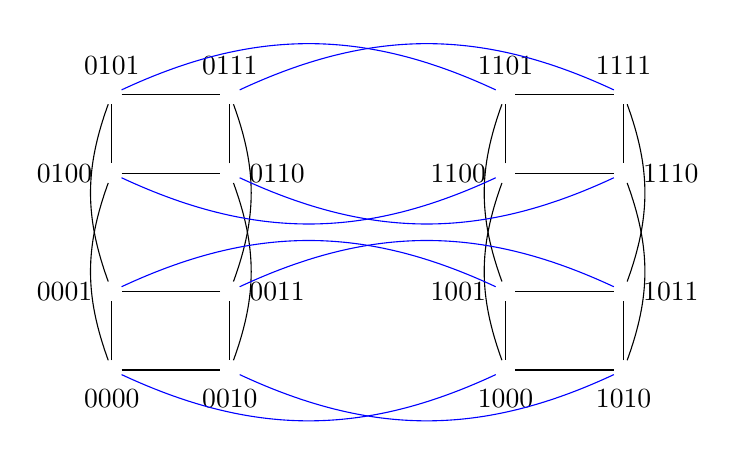
\begin{tikzpicture} 

\node[] at (0,0) [label=below:$0000$] (0000) {}; 
\node[] at (0,1) [label=left:$0001$] (0001) {}; 
\node[] at (1.5,0) [label=below:$0010$] (0010) {}; 
\node[] at (1.5,1) [label=right:$0011$] (0011) {}; 
\node[] at (0,2.5) [label=left:$0100$] (0100) {}; 
\node[] at (0,3.5) [label=above:$0101$] (0101) {}; 
\node[] at (1.5,2.5) [label=right:$0110$] (0110) {}; 
\node[] at (1.5,3.5) [label=above:$0111$] (0111) {}; 

\node[] at (5,0) [label=below:$1000$] (1000) {}; 
\node[] at (5,1) [label=left:$1001$] (1001) {}; 
\node[] at (6.5,0) [label=below:$1010$] (1010) {}; 
\node[] at (6.5,1) [label=right:$1011$] (1011) {}; 
\node[] at (5,2.5) [label=left:$1100$] (1100) {}; 
\node[] at (5,3.5) [label=above:$1101$] (1101) {}; 
\node[] at (6.5,2.5) [label=right:$1110$] (1110) {}; 
\node[] at (6.5,3.5) [label=above:$1111$] (1111) {}; 

\path (0000) 
edge (0001) 
edge (0010) 
edge [out=110, in=250](0100)
(0011)	
edge (0001) 
edge (0010) 
edge [out=70, in=-70] (0111)
(1111)	
edge (1110) 
edge (1101)
(0101)
edge (0111)
edge (0100)
edge [out=250, in=-250] (0001)
(1010)
edge (1000)
edge [out=70, in=-70] (1110)
edge (1011)
(0100)
edge (0110)
(0110)
edge (0111)
(1100)
edge (1101)
edge (1110)
edge [out=250, in=-250] (1000)
(1001)
edge (1000)
edge (1011)
edge [out=110, in=250] (1101)
	(0010)
	edge [out=70, in=-70] (0110)
	(1011)
	edge [out=70, in=-70] (1111);

	\path [blue]
	(0000)
	edge [out=-25,in=-155] 	(1000)
	(0010)
	edge [out=-25, in=-155] (1010)
	(0100)
	edge [out=-25, in=-155] (1100)
	(0110)
	edge [out=-25, in=-155] (1110)
	(0001)
	edge [out=25,in=155](1001)
	(0011)
	edge [out=25,in=155] (1011)
	(0101)
	edge [out=25,in=155] (1101) 
	(0111)
	edge [out=25,in=155] (1111);

	\end{tikzpicture}
\end{document}